\usepackage[utf8]{inputenc}
\usepackage[english,russian]{babel}
\usepackage[14pt]{extsizes}

%\usepackage{pscyr}
\usepackage{subfigure}
\usepackage{wrapfig}
\usepackage{cmap}
\usepackage{indentfirst}
\usepackage{autonum}
\usepackage{amsfonts}
\usepackage{amsmath}
\usepackage{amssymb}
\usepackage{amsthm}
\usepackage{upgreek}
\usepackage{graphicx}
\usepackage{listings}
\usepackage{multirow}
\usepackage{multicol}
\usepackage{dsfont}
\usepackage{graphicx}
\usepackage{caption}
\usepackage{setspace,amsmath}

\usepackage[unicode, pdftex]{hyperref}
\usepackage[left=30mm, top=20mm, right=15mm, bottom=20mm, footskip=10mm]{geometry}
\usepackage{xcolor}

\definecolor{maroon}{cmyk}{0, 0.87, 0.68, 0.32}
\definecolor{halfgray}{gray}{0.55}
\definecolor{ipython_frame}{RGB}{207, 207, 207}
\definecolor{ipython_bg}{RGB}{247, 247, 247}
\definecolor{ipython_red}{RGB}{186, 33, 33}
\definecolor{ipython_green}{RGB}{0, 128, 0}
\definecolor{ipython_cyan}{RGB}{64, 128, 128}
\definecolor{ipython_purple}{RGB}{170, 34, 255}

\usepackage{listings}
\lstset{
    breaklines=true,
    texcl=true,
    %
    extendedchars=true,
    literate=
    {á}{{\'a}}1 {é}{{\'e}}1 {í}{{\'i}}1 {ó}{{\'o}}1 {ú}{{\'u}}1
    {Á}{{\'A}}1 {É}{{\'E}}1 {Í}{{\'I}}1 {Ó}{{\'O}}1 {Ú}{{\'U}}1
    {à}{{\`a}}1 {è}{{\`e}}1 {ì}{{\`i}}1 {ò}{{\`o}}1 {ù}{{\`u}}1
    {À}{{\`A}}1 {È}{{\'E}}1 {Ì}{{\`I}}1 {Ò}{{\`O}}1 {Ù}{{\`U}}1
    {ä}{{\"a}}1 {ë}{{\"e}}1 {ï}{{\"i}}1 {ö}{{\"o}}1 {ü}{{\"u}}1
    {Ä}{{\"A}}1 {Ë}{{\"E}}1 {Ï}{{\"I}}1 {Ö}{{\"O}}1 {Ü}{{\"U}}1
    {â}{{\^a}}1 {ê}{{\^e}}1 {î}{{\^i}}1 {ô}{{\^o}}1 {û}{{\^u}}1
    {Â}{{\^A}}1 {Ê}{{\^E}}1 {Î}{{\^I}}1 {Ô}{{\^O}}1 {Û}{{\^U}}1
    {œ}{{\oe}}1 {Œ}{{\OE}}1 {æ}{{\ae}}1 {Æ}{{\AE}}1 {ß}{{\ss}}1
    {ç}{{\c c}}1 {Ç}{{\c C}}1 {ø}{{\o}}1 {å}{{\r a}}1 {Å}{{\r A}}1
    {€}{{\EUR}}1 {£}{{\pounds}}1
}

%%
%% Python definition (c) 1998 Michael Weber
%% Additional definitions (2013) Alexis Dimitriadis
%% modified by me (should not have empty lines)
%%
\lstdefinelanguage{iPython}{
    morekeywords={access,and,break,class,continue,def,del,elif,else,except,exec,finally,for,from,global,if,import,in,is,lambda,not,or,pass,print,raise,return,try,while},%
    %
    % Built-ins
    morekeywords=[2]{abs,all,any,basestring,bin,bool,bytearray,callable,chr,classmethod,cmp,compile,complex,delattr,dict,dir,divmod,enumerate,eval,execfile,file,filter,float,format,frozenset,getattr,globals,hasattr,hash,help,hex,id,input,int,isinstance,issubclass,iter,len,list,locals,long,map,max,memoryview,min,next,object,oct,open,ord,pow,property,range,raw_input,reduce,reload,repr,reversed,round,set,setattr,slice,sorted,staticmethod,str,sum,super,tuple,type,unichr,unicode,vars,xrange,zip,apply,buffer,coerce,intern},%
    %
    sensitive=true,%
    morecomment=[l]\#,%
    morestring=[b]',%
    morestring=[b]",%
    %
    morestring=[s]{'''}{'''},% used for documentation text (mulitiline strings)
    morestring=[s]{"""}{"""},% added by Philipp Matthias Hahn
    %
    morestring=[s]{r'}{'},% `raw' strings
    morestring=[s]{r"}{"},%
    morestring=[s]{r'''}{'''},%
    morestring=[s]{r"""}{"""},%
    morestring=[s]{u'}{'},% unicode strings
    morestring=[s]{u"}{"},%
    morestring=[s]{u'''}{'''},%
    morestring=[s]{u"""}{"""},%
    %
    % {replace}{replacement}{lenght of replace}
    % *{-}{-}{1} will not replace in comments and so on
    literate=
    {á}{{\'a}}1 {é}{{\'e}}1 {í}{{\'i}}1 {ó}{{\'o}}1 {ú}{{\'u}}1
    {Á}{{\'A}}1 {É}{{\'E}}1 {Í}{{\'I}}1 {Ó}{{\'O}}1 {Ú}{{\'U}}1
    {à}{{\`a}}1 {è}{{\`e}}1 {ì}{{\`i}}1 {ò}{{\`o}}1 {ù}{{\`u}}1
    {À}{{\`A}}1 {È}{{\'E}}1 {Ì}{{\`I}}1 {Ò}{{\`O}}1 {Ù}{{\`U}}1
    {ä}{{\"a}}1 {ë}{{\"e}}1 {ï}{{\"i}}1 {ö}{{\"o}}1 {ü}{{\"u}}1
    {Ä}{{\"A}}1 {Ë}{{\"E}}1 {Ï}{{\"I}}1 {Ö}{{\"O}}1 {Ü}{{\"U}}1
    {â}{{\^a}}1 {ê}{{\^e}}1 {î}{{\^i}}1 {ô}{{\^o}}1 {û}{{\^u}}1
    {Â}{{\^A}}1 {Ê}{{\^E}}1 {Î}{{\^I}}1 {Ô}{{\^O}}1 {Û}{{\^U}}1
    {œ}{{\oe}}1 {Œ}{{\OE}}1 {æ}{{\ae}}1 {Æ}{{\AE}}1 {ß}{{\ss}}1
    {ç}{{\c c}}1 {Ç}{{\c C}}1 {ø}{{\o}}1 {å}{{\r a}}1 {Å}{{\r A}}1
    {€}{{\EUR}}1 {£}{{\pounds}}1,
    %
    literate=
    *{+}{{{\color{ipython_purple}+}}}1
    {-}{{{\color{ipython_purple}-}}}1
    {*}{{{\color{ipython_purple}$^\ast$}}}1
    {/}{{{\color{ipython_purple}/}}}1
    {^}{{{\color{ipython_purple}\^{}}}}1
    {?}{{{\color{ipython_purple}?}}}1
    {!}{{{\color{ipython_purple}!}}}1
    {\%}{{{\color{ipython_purple}\%}}}1
    {<}{{{\color{ipython_purple}<}}}1
    {>}{{{\color{ipython_purple}>}}}1
    {|}{{{\color{ipython_purple}|}}}1
    {\&}{{{\color{ipython_purple}\&}}}1
    {~}{{{\color{ipython_purple}~}}}1
    %
    {==}{{{\color{ipython_purple}==}}}2
    {<=}{{{\color{ipython_purple}<=}}}2
    {>=}{{{\color{ipython_purple}>=}}}2
    %
    {+=}{{{+=}}}2
    {-=}{{{-=}}}2
    {*=}{{{$^\ast$=}}}2
    {/=}{{{/=}}}2,
    %
    commentstyle=\color{ipython_cyan}\ttfamily,
    stringstyle=\color{ipython_red}\ttfamily,
    keepspaces=true,
    showspaces=false,
    showstringspaces=false,
    rulecolor=\color{ipython_frame},
    frame=single,
    frameround={t}{t}{t}{t},
    framexleftmargin=6mm,
    numbers=left,
    numberstyle=\tiny\color{halfgray},
    %
    backgroundcolor=\color{ipython_bg},
    % extendedchars=true,
    basicstyle=\scriptsize\ttfamily,
    keywordstyle=\color{ipython_green}\ttfamily,
    escapechar=\%,
    escapebegin=\color{ipython_green},
    texcl=true,
    inputencoding=utf8
}

\begin{document}
	\selectlanguage{russian}
\setcounter{page}{0}

\begin{center}
	\small{Министерство науки и высшего образования Российской Федерации}\\
	\small{Федеральное государственное бюджетное образовательное учреждение}\\
	\small{Высшего образования}\\
	\small{\textbf{«Северо-Осетинский государственный университет\\
			имени Коста Левановича Хетагурова»}}\\
	
	\hfill \break
	\hfill \break
	\hfill \break
	\hfill \break
	\hfill \break
	\hfill \break
	\hfill \break
	\hfill \break
	\hfill \break
	\hfill \break
	\hfill \break
	\hfill \break
	\hfill \break
	
	\normalsize{Дипломная работа}\\
	\large{\textbf{Seq2Seq - подход для реализации машинного перевода}}\\
	
	\hfill \break
	\hfill \break
	\hfill \break
	\hfill \break
	\hfill \break
	\hfill\break
\end{center}

\begin{flushright}
	\textbf{Выполнил:}\\
	Студент 4 курса направления:\\
	«Прикладная математика и информатика»\\
	\textit{Гамосов Cтанислав Станиславович \underline{\hspace{3cm}}}\\
\end{flushright}

\hfill

\begin{flushright}
	\textbf{Научный руководитель:}\\
	Кандидат физико-математических наук:\\
	\textit{Басаева Елена Казбековна \underline{\hspace{3cm}}}\\
\end{flushright}

\hfill

\begin{flushright}
	\textbf{Консультант}\\
	Старший преподаватель: \\
	\textit{Макаренко Мария Дмитриевна \underline{\hspace{3cm}}}\\
\end{flushright}

\normalsize{ \hspace{28pt}} \hfill \break
\begin{center} Владикавказ 2022 \end{center}
\thispagestyle{empty}
\clearpage
	\thispagestyle{empty}
\tableofcontents
\thispagestyle{empty}
\clearpage
\newtheorem{theorem}{Теорема}
	
	\section{Введение}
	
	За последние годы качество моделей машинного перевода резко выросло, связано это с началом использования в них рекуррентных нейронных сетей (RNN). Они позволили снизить затраты на выявления лингвистических закономерностей языков и дорогостоящую разработку алгоритмов для их обработки, что использовалось в RBMT (Rule-Based Machine Translation). В свою очередь NMT (Neural Machine Translation) довольно хорошо справляется со своей задачей, но все таки ему не удалось полностью сместить SMT (Statistical Machine Translation). Количество статистического перевода в современных переводчиках снизилось почти до минимума. Теперь уже при построении хорошей модели машинного перевода большую часть работы стоит с концентрировать, на особенности языка, его структуре, связи между словами и их значениями. Решения данного перечня проблем и являются модели sequence-to-sequence (\cite{10}, \cite{11}, \cite{12}).
	
	Seq2Seq - это семейство подходов машинного обучения, используемых для обработки языка. Нейронный перевод, текстовое описание к изображению и обобщение (summarize) текста - вот не полный список задач, в которых используются данная модель.
	
	Первоначальный подход Seq2Seq, который в процессе породил целое семейство методов, был разработан Google для использования в машинном переводе \cite{21}. Как уже можно заметить за последнюю пару лет коммерческие системы стали удивительно хороши в переводе - посмотрите, например, Google Translate, Яндекс-Переводчик, переводчик DeepL, переводчик Bing Microsoft.
	
	Однако, не стоит думать, что данная технология применяется, только в обработки естественных языков. Она несет в себе огромный потенциал, помимо привычного машинного перевода, вполне реализуем перевод между языками программирования (Facebook AI - Глубокое обучение переводу между языками программирования \cite{19}). Возможности применений такого рода подходов довольно велики. В связи с этим под машинным переводом можно подразумевать любую задачу в переводе одной последовательности в любую другую.
	
	\clearpage
	
	\section{Рекуррентные сети}
	
	\subsection{RNN - Recиrrent Neural Network}
	
	\textit{Рекуррентные Нейронные Сети} (RNN - Recиrrent Neural Network) - это нелинейная динамическая система, которая сопоставляет последовательности с последовательностями. Основная философия заключается, в том что мысли обладают неким постоянством и напрямую зависят от прошлых умозаключений \cite{20}. 
	
	RNN способны работать с последовательностями произвольной длины, а не с входными данными фиксированного размера. Это свойство как раз таки очень важно в контексте обработки естественных языков. Так же весомое отличие таких сетей от обычных это понятие времени. Под ним подразумевается последовательность входных данных $x_t$, которая поступает на вход, и их выходная последовательность $y_t$, которые генерируются на основе дискретной входной последовательности. 
	
	Для большего понимания данной абстракции, давайте рассмотрим один конкретный пример. Допустим мы изучаем траекторию полета баскетбольного мяча и главный вопрос: «Попадет ли он в корзину или нет?». Для решение поставленной задачи нужно знать направление движения мяча. Имея только такую информацию вы можете пойти дальше и сделать предположение. Однако любой ответ является просто случайным предположением. Не имея информации, где находится баскетбольный мяч, у вас не будет достаточно данных, чтобы предсказать, куда он попадет. В свою очередь если поставить камеру и сделать много снимков во время полета мяча и расставить их перед собой в ряд, прогноз улучшится, так как вы обладаете большим количеством информации и контекста.
	
	Как уже говорилось, в результате получаемые последовательности могут быть конечной длины или бесконечно счетными. Таким образом, входную последовательность можно обозначить за $x = (x_0, x_1, x_2, ... , x_t)$, а выходную последовательность как $y = (y_0, y_1, y_2, ... , y_t)$
	
	\begin{figure}[ht!]
		\centering
		\captionsetup{justification=centering}
		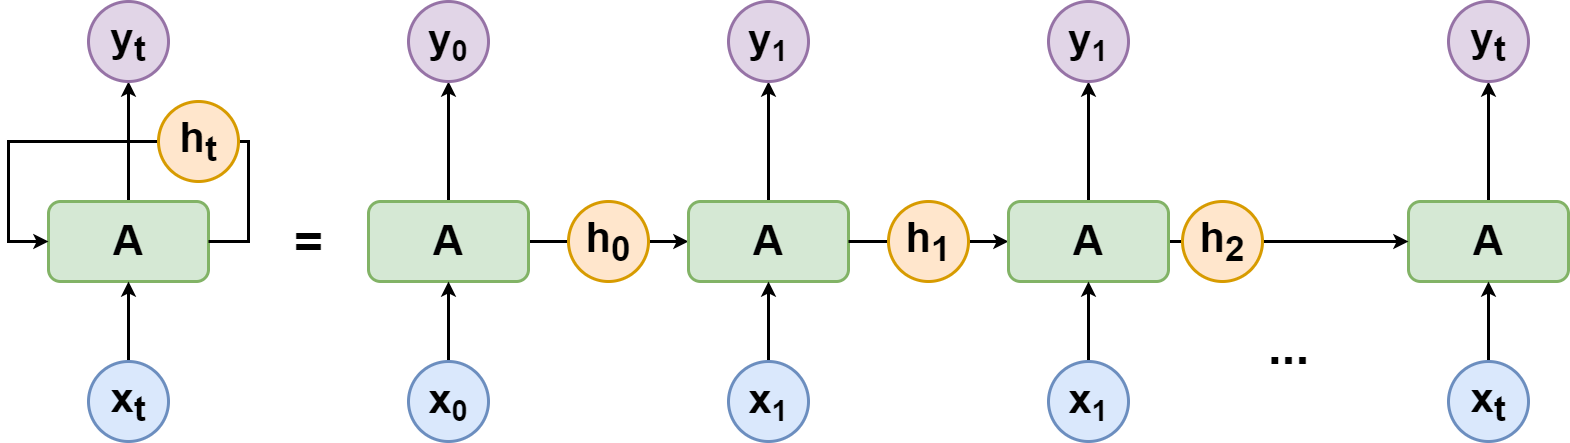
\includegraphics[height=40mm]{img/RNN и ее развернутое представление.png}
		\caption{RNN и ее развернутое представление}
	\end{figure}
	
	Нейронная сеть $A$ принимает входной вектор $x_t$ и после обработки получается выходной вектор $y_t$. RNN обрабатывает входную последовательность, имея рекуррентные скрытые состояния $h_t$, активация которых в каждый момент времени зависит от активации в предыдущие разы.
	
	Обычно обновление повторно скрытого состояния реализуется по такой формуле\cite{3}:
	
	\begin{equation}
        h_t = 
        \begin{cases}
            0 & \text{t = 0}\\
            \sigma(W x_t + U h_{t - 1}) & \text{иначе}
        \end{cases}
    \end{equation}
    
    где $W$, $U$ - матрицы весов, $\sigma$ - функция активации.
    
    \textit{Вес} - это связь между вершинами, которая несет в себе число, характеризующее важность, передаваемого значения, проходящего через данное ребро. Для пары узлов $i$ (узел входного слоя) и $j$ (узел скрытого слоя) присутствует собственный вес $w_{ij}$. Легче всего это представить как матрицу смежности $W$, где на пересечение $i$ строки и $j$ столбца находятся числа отвечающие за вес. Такая же матрица только для скрытого слоя в выходной слоя будем обозначаться $U$. 
    
    \textit{Функция активации} - является абстракцией, представляющей степень возбуждения нейрона. Определяет выходное значение нейрона в зависимости от результата взвешенной суммы входов и значения скрытых слоев ($W x_t + U h_{t - 1}$). \cite{20}
	
	Развернув рекуррентную сеть можно легко представить её, как копий одной и той же сети, каждая из которых передает информацию последующей копии. В таком виде RNN довольно просто интерпретировать как временную последовательность. На сегодняшний день рекуррентные сети - самая естественная архитектура нейронных сетей для работы с данными такого типа. 
	
	\subsection{Elman and Jordan Networks}
	
	Для большего понимания рекуррентных сетей рассмотрим, пару конкретных реализаций. \textit{Нейронная сеть Элмана} - это нейронная сеть, состоящая из трёх слоев. Первый слой $x_t$ - является входным вектором, а $y_t$ вектором выходного слоя. Слой $h_t$ - напрямую отвечает за скрытое состояние сети. В дополнение к обычной RNN добавлен новый блок $c$. Его называют \textit{контекстным блоком}. Скрытый слой $h$ соединён с контекстными блоками $c$ фиксированным весом, которого равен единице.
	
	С каждым шагом времени на вход $x$ поступает информация, которая проходит прямой ход к выходному слою $y$ в соответствии с правилами обучения. Фиксированные обратные связи сохраняют предыдущие значения скрытого слоя $h$ в контекстных блоках $c$ (до того как скрытый слой поменяет значение в процессе обучения). Таким способом сеть сохраняет своё состояние, что может использоваться в предсказании последовательностей.
	
	\begin{table}[h]
		\centering
		\begin{tabular}{|c|} 
			\hline
			\textbf{Elman Networks}  \\ 
			\hline
			$ h_{t} = \sigma_{h}(W_h x_t + U_h h_{t - 1} + b_h) $ \\ 
			$ y_{t} = \sigma_{y}(W_y h_t + b_y) $ \\
			\hline
		\end{tabular}
	\end{table}
	\begin{tabbing}
		$x_t$, $h_t$, $y_t$  - векторы входного, скрытого, выходного слоя \\
		$W$, $U$ и $b$ - матрицы и вектор параметров \\
		$\sigma_h$ и $\sigma_y$ - функции активации
	\end{tabbing}
    
    Так же стоит рассмотрим вторую именную архитектуру RNN. \textit{Сеть Джордана} - трехслойная нейронная сеть. Единственное отличие между сетью Элмана - это обновления контекстного блока. Контекстные блоки $c$ связаны не со скрытым слоем $h$, а с выходным слоем $y$. Они обладают рекуррентной связью с собой.
    
    \begin{table}[h]
		\centering
		\begin{tabular}{|c|} 
			\hline
			\textbf{Jordan Networks}  \\ 
			\hline
			$	h_{t} = \sigma_{h}(W_h x_t + U_h y_{t - 1} + b_h) $  \\
			$	y_{t} = \sigma_{y}(W_y h_t + b_y) $ \\
			\hline
		\end{tabular}
	\end{table}
	\begin{tabbing}
		$x_t$, $h_t$, $y_t$  - векторы входного, скрытого, выходного слоя \\
		$W$, $U$ и $b$ - матрицы и вектор параметров \\
		$\sigma_h$ и $\sigma_y$ - функции активации
	\end{tabbing}
	
    \begin{figure}[h]
		\centering
		\captionsetup{justification=centering}
		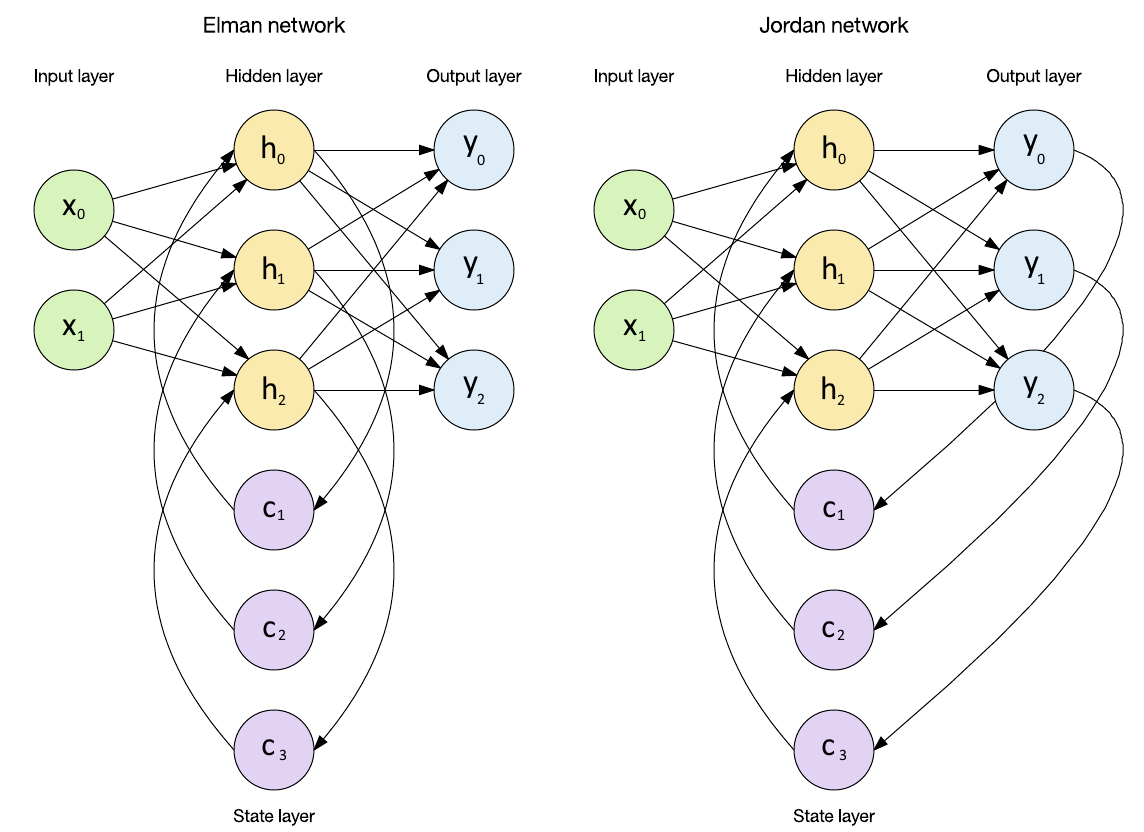
\includegraphics[width=0.98\textwidth]{img/RNN.png}
		\caption{Схемы архитектур RNN}
	\end{figure}
	
	\subsection{Проблема долговременных зависимостей}
	
	Довольно весомый плюс RNN является, то что нейронная сеть хорошо справляется с построением связей между предыдущей информацией и поставленной задачей. Данное свойство можно наглядно увидеть на рассмотренном примере, выше, про баскетбольный мяч. Однако выяснилось, что не всегда RNN справляется с такой проблемой \cite{2}. Это зависит от некоторых обстоятельств.

	В процессе работы с RNN было замечено, что в случае, когда дистанция между актуальной информацией и местом, где она понадобилась, велика, то сети могут могут забыть нужную информацию из прошлого \cite{2}. Долгосрочные зависимости плохо воспринимаются обычными рекурсивными сетями, потому что градиенты имеют тенденцию либо исчезать, либо взрываться. Это затрудняет метод оптимизации на основе градиента не только из-за различий в величинах, но и из-за того, что эффект долгосрочных зависимостей скрыт эффектом краткосрочных зависимостей. 
	
	Один из подходов, который решает текущую проблему, заключается в разработке более сложной функции активации, чем обычные функции что применялись ранее в реализация Элмана и Джордона \cite{1}, \cite{4}. Самая ранняя попытка в этом направлении привела к появлению нового управляемого рекуррентного блока, называемого блоком долгой краткосрочной памяти (LSTM)\cite{2}. Со временем данная архитектура была улучшена и появился более современный тип управляемых рекуррентных сетей (GRNN - Gated Recurrent Neural Networks) - это управляемые рекуррентные блоки (GRU)\cite{3}. Было показано, что некоторые из этих повторяющихся блоков хорошо справляются с задачами, требующими учета долгосрочных зависимостей.
	
	\subsection{GRNN - Gated Recurrent Neural Networks}
	\subsubsection{LSTM - Long Short-Term Memory}
	
	Сети долгой краткосрочной памяти (LSTM) - особая разновидность архитектуры RNN, способная к обучению долговременным зависимостям. Они были представлены Зеппом Хохрайтер и Юргеном Шмидхубером в 1997 \cite{2}. Любая рекуррентная нейронная сеть представима в форме рекуррентной последовательности повторяющихся блоков нейронной сети. Как уже было сказано, обычная RNN можно представить в виде одного слоя с любой функцией активации, например $tanh$. 
	
	\begin{figure}[ht!]
		\centering
		\captionsetup{justification=centering}
		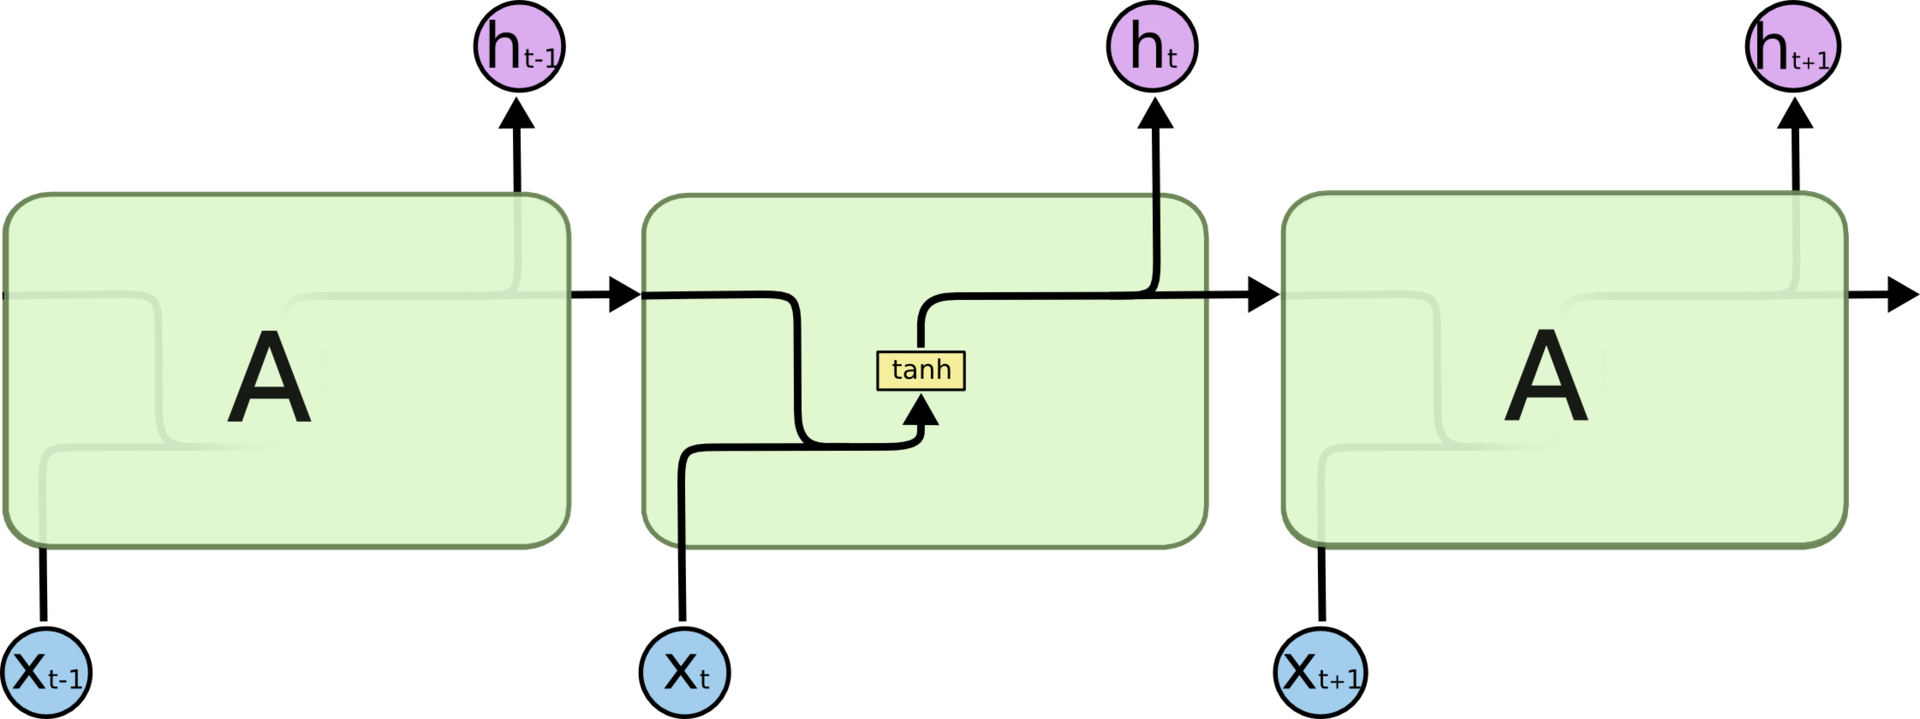
\includegraphics[width=0.8\textwidth]{img/RNN Chain.png}
		\caption{Повторяющийся блок стандартной RNN}
	\end{figure}
	
	Обозначим специальные обозначения, которые будут использоваться в схемах.
	\begin{figure}[ht!]
		\centering
		\captionsetup{justification=centering}
		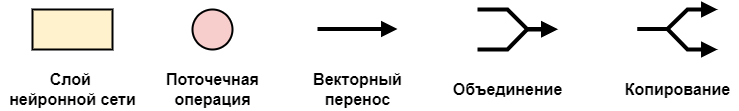
\includegraphics[width=0.65\textwidth]{img/Обозначения.png}
	\end{figure}
	
	Структура LSTM как и RNN представляет друг за другом идущие блоки, но сама структура блоков сильно отличается. Вместо одного слоя нейронной сети с его функцией активации блоки содержат целых четыре слоя.
	
	\begin{figure}[ht!]
		\centering
		\captionsetup{justification=centering}
		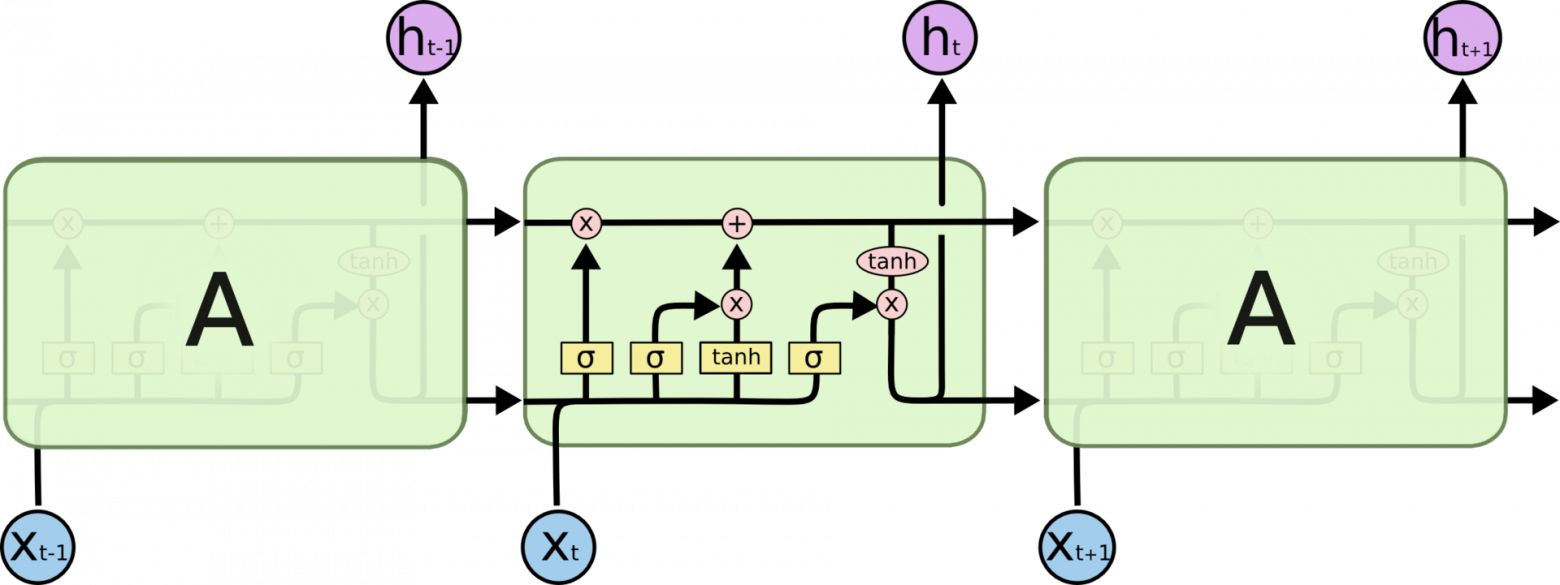
\includegraphics[width=0.8\textwidth]{img/LSTM Chain.png}
		\caption{Схема блоков LSTM}
	\end{figure}
	
	Главное нововведение LSTM – это ячейки состояния $C_t$ (cell state). На схеме обозначена, как горизонтальная линия, проходящая по верхней части блока.
	
	Ячейка состояния напоминает конвейерную ленту. Она проходит напрямую через всю цепочку, участвуя лишь в нескольких линейных преобразованиях. Информация может легко передаваться по ней без изменений.
	
	\begin{figure}[h]
		\centering
		\captionsetup{justification=centering}
		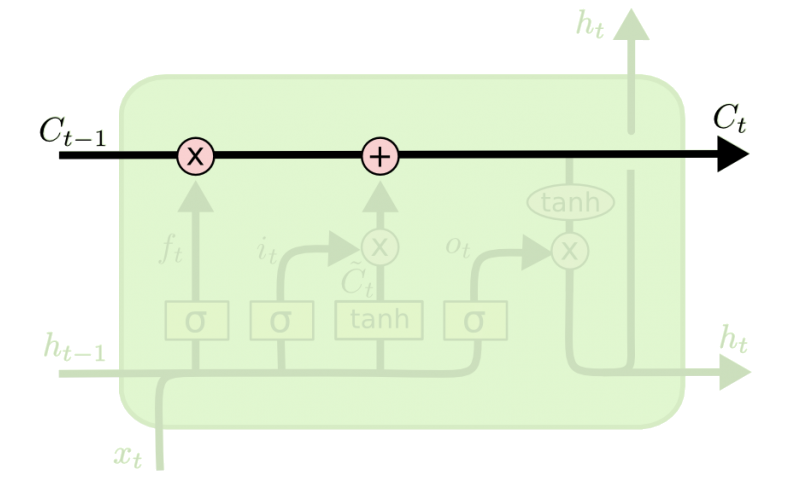
\includegraphics[width=0.6\textwidth]{img/LSTM 1.png}
		\caption{«Лента» ячейки состояния}
	\end{figure}
	
	Однако, LSTM может спокойно удалять информацию из ячейки состояния. Этот механизм управляется и регулируется фильтрами (gates). Фильтры позволяют пропускать информацию на основании некоторых условий. Они состоят из слоя сигмоидальной нейронной сети и операции поэлементного умножения.
	
	\begin{figure}[h]
		\centering
		\captionsetup{justification=centering}
		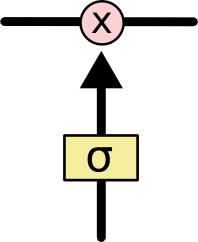
\includegraphics[width=0.15\textwidth]{img/Gates.png}
		\caption{Схема фильтра LSTM}
	\end{figure}
	
	За счет сигмоиды слой возвращает числа в отрезке [0,1], которые обозначают, какую долю каждого блока информации следует пропустить дальше по сети. 0 - означает \textit{не пропускать ничего}, 1 - \textit{пропустить все}.
    
    Более подробно механизм LSTM работает так: на первом шагу нужно определить, какую информацию стоит выбросить из ячейки состояния. Это решение принимает слой на котором применяем сигмойду, называемый \textit{слоем фильтра забывания} (forget gate layer). Данный слой берет $h_{t-1}$ и $x_t$ конкретизирует их и возвращает $f_t$ число от 0 до 1 для каждого числа из состояния ячейки $C_{t-1}$.
    
    \begin{figure}[ht!]
		\centering
		\captionsetup{justification=centering}
		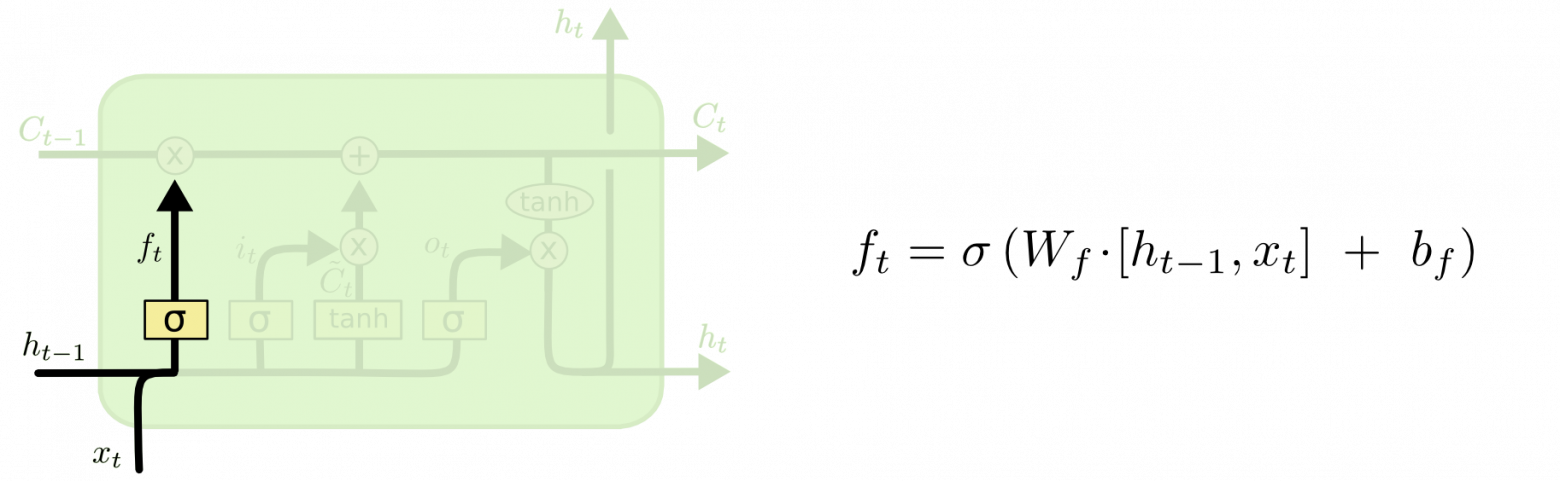
\includegraphics[width=0.92\textwidth]{img/LSTM_step1.png}
	\end{figure}
	
	Следующий шаг определить какая новая информация будет храниться в ячейки состояний. На данном этапе участвуют два слоя. \textit{Слой входного фильтра} (input layer gate) - это сигмоидальный слой определяет, какие значения следует обновить. Второй слой имеет внутри себя функцию активации $tanh$. Этот $tanh$-слой строит вектор новых значений-кандидатов $\tilde{C}_t$.
    
    \begin{figure}[h]
		\centering
		\captionsetup{justification=centering}
		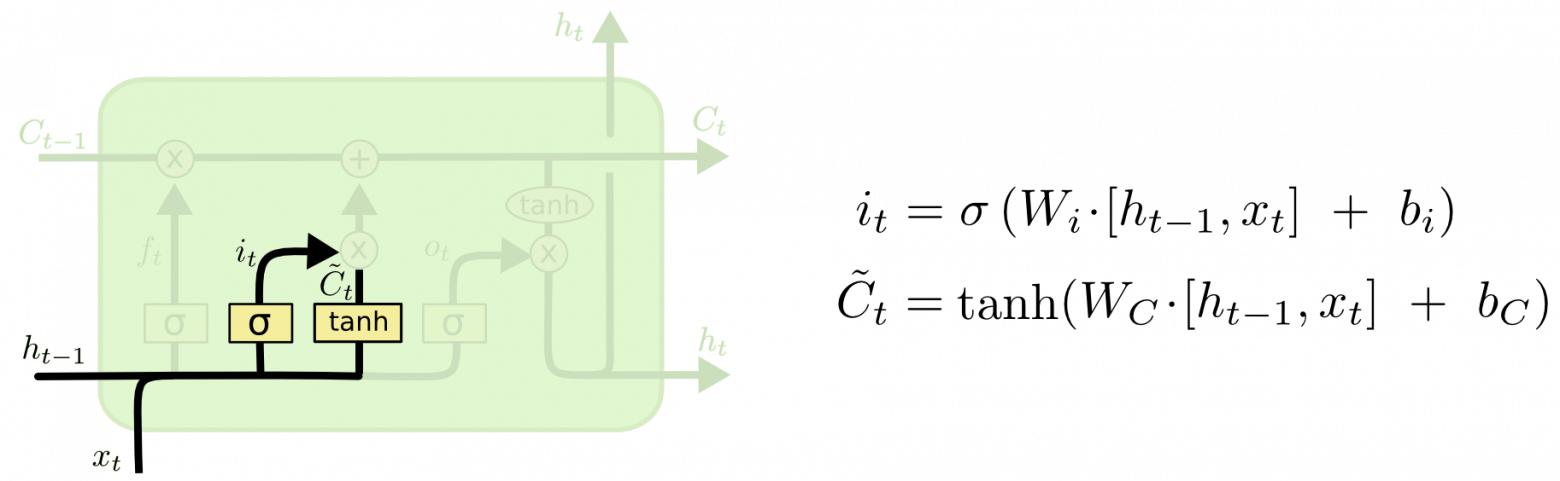
\includegraphics[width=0.92\textwidth]{img/LSTM_step2.png}
	\end{figure}
	
    После всех преобразований необходимо заменить старые ячейки состояний $C_{t-1}$ на новые $C_t$. Умножив старые состояния на $f_t$, тем самым мы забываем ту информацию, которая нам не нужна. Следующим шагом к полученному поэлементно прибавляем преобразованные выходные слои $i_t \otimes \tilde{c}_t$ ($\otimes$ - поэлементное умножение). Новые значения-кандидаты $\tilde{C_t}$, поэлементно умноженные на $i_t$ – на сколько мы хотим обновить каждое из значений состояния.

    \begin{figure}[h]
		\centering
		\captionsetup{justification=centering}
		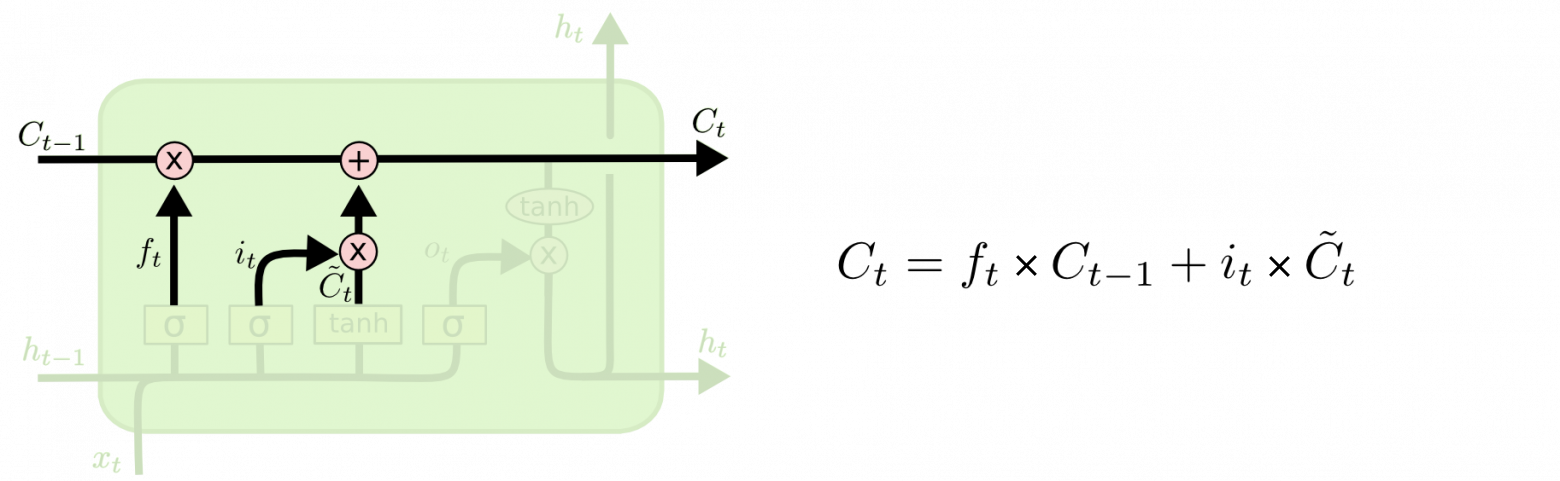
\includegraphics[width=0.92\textwidth]{img/LSTM_step3.png}
	\end{figure}
	
	Последним шагом, нужно определить, какую информацию мы хотим получать на выходе. Выходной слой (output layer gate) будут основаны на наших скрытых слоях, к ним будут применены некоторые фильтры. Для начала применим сигмоидальный слой, который решит, какую информацию из скрытых состояний нужно выводить. Затем нужно новые значения ячеек состояния прогнать через активацию $tanh$, чтобы получить на выходе значения из диапазона [-1, 1]. Полученный результат надо перемножить с выходными значениями сигмоидального слоя.

    \begin{figure}[ht!]
		\centering
		\captionsetup{justification=centering}
		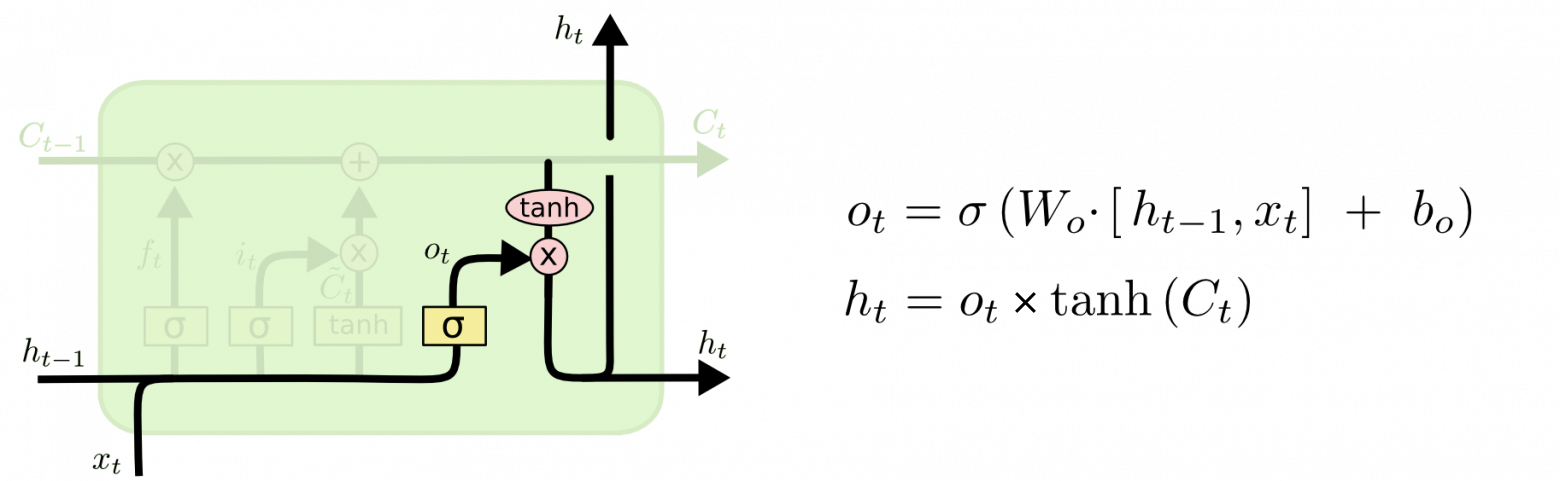
\includegraphics[width=0.92\textwidth]{img/LSTM_step4.png}
	\end{figure}
	
	В отличие от обычных RNN, которые перезаписывают свое содержимое на каждом шаге времени, блок LSTM способен решать, следует ли сохранять существующую состояния или нет с помощью введенных элементов. Интуитивно понятно, что если модуль LSTM обнаруживает важную функцию из входной последовательности на ранней стадии, он легко переносит эту информацию на большие расстояния, следовательно, фиксируя потенциальные зависимости \cite{2}.
	
	\subsubsection{GRU - Gated Recurrent Unit}
	
	Управляемые рекуррентные блоки была предложена в 2014 \cite{3}. Аналогично блоку LSTM, GRU имеет фильтры, которые модулируют поток информации внутри блока, однако, не имеет отдельные ячейки состояния.
	
    GRU избавилось от ячеек состояния и использует скрытое состояние для передачи информации. Эта архитектура имеет только два фильтра, фильтр сброса и фильтр обновления.
    
    \textit{Слой фильтра обновления} (update layer gate) элемент обновления действует аналогично слоям входного и выходного фильтра в LSTM. Он решает, какую информацию выбросить и какую новую информацию добавить.
    
    \textit{Слой фильтра сброса} (reset layer gate) - это еще один элемент, который используется для определения того, сколько предыдущей информации следует забыть.
    
    У GRU меньше операций, следовательно, обучение такой архитектуры немного быстрее, чем у LSTM \cite{4}. Однако точно сказать, кто явный победитель, довольно затруднительно.
    
    \begin{figure}[ht!]
		\centering
		\captionsetup{justification=centering}
		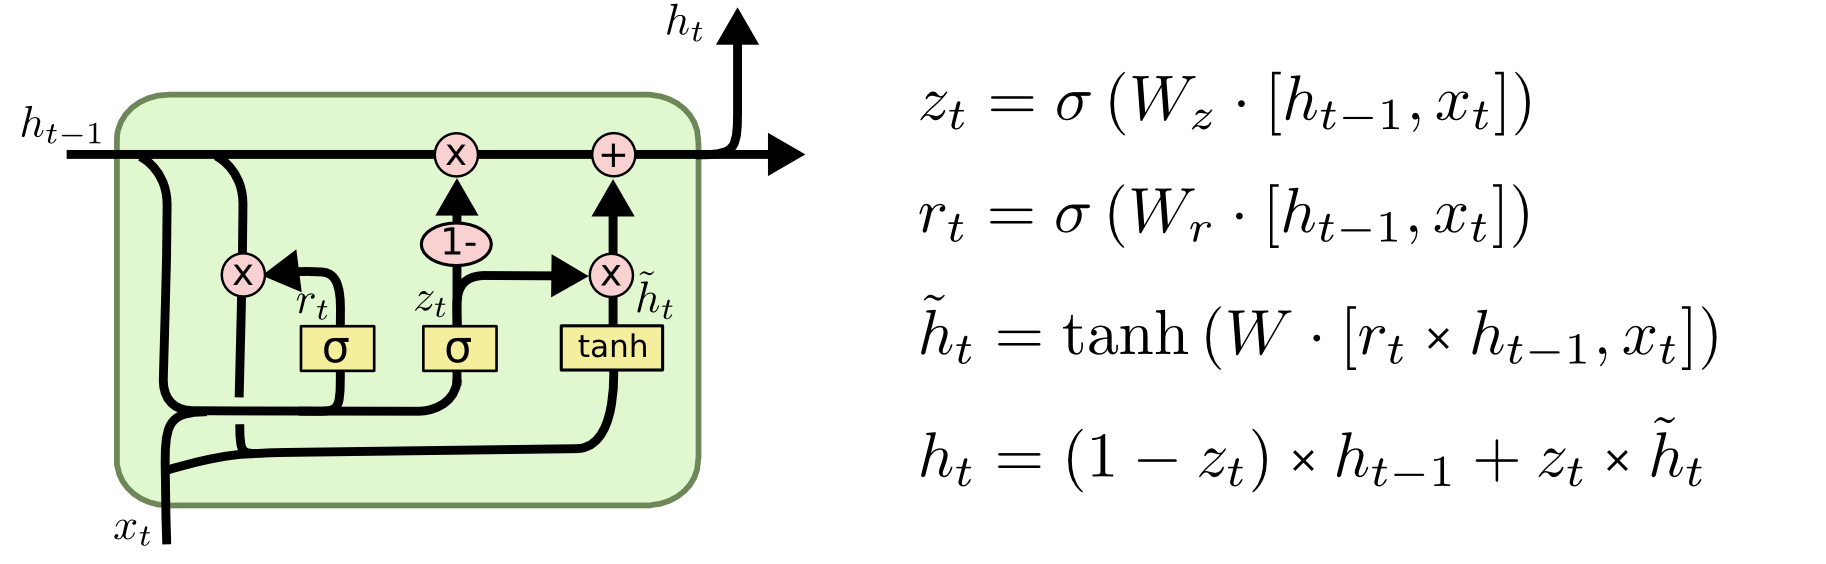
\includegraphics[width=0.92\textwidth]{img/GRU.png}
	\end{figure}
	
	\clearpage
 	
	\section{Задача машинного перевода}
	
	Нейронный машинный перевод (NMT, Neural Machine Translation) - это радикальное изменение подходов к машинному переводу. С одной стороны, NMT использует непрерывные представления вместо дискретных символьных представлений. С другой стороны, NMT использует единую большую нейронную сеть для моделирования всего процесса перевода, избавляя от необходимости чрезмерного проектирования функций. Помимо своей простоты, NMT добился высочайшей производительности на различных языковых парах. На практике же NMT также становится ключевой технологией многих коммерческих систем, как уже было сказано выше.
	
	В качестве подхода к машинному переводу, основанного на данных, NMT использует вероятностную структуру. С математической точки зрения, цель NMT состоит в том, чтобы оценить неизвестное условное распределение $P(y|x)$ с учетом набора данных $\mathcal{D}$, где $x$ и $y$ - случайные величины, представляющие исходный ввод и целевой вывод соответственно.
	
    Переводить можно последовательность на разных уровнях. В качестве единицы перевода можно взять предложения, абзацы или тексты. В статье основной единицей будет являться предложение. Благодаря такому уточнению, модель NMT можно рассматривать как модель sequence-to-sequence. 
    
    На вход подается предложение $X = \{x_1, x_2, ... , x_T\}$ и целевое предложений $Y = \{y_1, x_2, ... , y_T\}$. Благодаря таким обозначениям, можно рассматривать перевод как нахождение целевой последовательности, которая является наиболее вероятной с учетом входных данных. Если более формально, то задача состоит в том, чтобы найти целевую последовательность, которая максимизирует условную вероятность $P(y|x)$. Однако этого не достаточно, нужен еще некоторый параметр $\theta$, от который и будет изменяться условная вероятность в процессе обучения. 
    
    $$
        y' = \text{arg max}_y P(y = Y | x = X; \theta)
    $$
    
    Таким образом, чтобы построить модель машинного перевода, нам нужно ответить на три вопроса:
    
    \begin{enumerate}
        \item Моделирование - Как выглядит модель для $P(y|x; \theta)$?
        \item Обучение - Как найти параметры $\theta$?
        \item Вывод - Как найти «лучший» $y$?
    \end{enumerate}
    
    \subsection{Моделирование}

        Почти все модели нейронного машинного перевода используют стандартную парадигму Encoder-Decoder. Такая структура состоит из четырех основных компонентов: слоя Embedding, сетей Encoder и Decoder и уровня Classification.
    
    Encoder - считывает исходную последовательность и создает ее представление. Decoder - использует исходное представление из Encoder для генерации целевой последовательности.
    
    Для однозначности конца и начала предложения в последовательностях используются токены начала последовательности (<sos> - start of sequence) и конца последовательности (<eos> - end of sequence), чтобы меньше отцентрировать внимания на разборе особенностях языков.
	
	Слой Embedding воплощает в себе сопоставление произвольной сущности (например, предложение или слово) некоторому вектору. Полученный дискретный результат обозначается как $x_t \in \mathbb{R}^d$, где $d$ - размерность вектора. Затем embedding отправляются в другие слои сети.
	
	Слой Encoder отображает исходный embedding в скрытое состояние $h_t$. Encoder должен уметь моделировать порядок и сложные зависимости, которые существовали в исходном языке. Рекуррентные нейронные сети (RNN) являются подходящим выбором для моделирования последовательностей переменной длины \cite{12}. Опишем RNNs вычисления, выполняемые в слои Encoder, как:
	
	$$
	    h_t = \text{EncoderRNN}(x_t, h_{t-1})
	$$
	
	В данном контексте под RNN может подразумеваться любая рекуррентная сеть. Например: LSTM \cite{2} или GRU \cite{3}.

	На каждом шаге итеративного процесса применяя полученную функцию $\text{EncoderRNN}$ к входной последовательности, можно в конечном случае получить скрытое состояние $h_S$ и использовать его в качестве представления для всей исходной последовательности (предложения). Затем передать его в Decoder.
	
	Decoder в свою же очередь можно рассматривать как языковую модель, зависящую от $h_S$. Сеть Decoder извлекает необходимую информацию из выходных данных слоя Encoder, а также моделирует зависимости на больших расстояниях между целевыми словами. Однако в процессе работы с RNN было замечено, что архитектуры LSTM и GRU хоть и справлялись с моделированием зависимостей и особенностей языка, но все равно уступали статическому переводу. Поэтому решение внедрения механизма Attention является важной вехой в исследованиях архитектуры NMT \cite{16}. Attention вычисляет релевантность каждого входного вектора значений на основе запросов и ключей (оригинальный перевод).
	
	Учитывая начальный элемент последовательности $y_0 = <sos>$ и скрытое состояние $s_0 = h_S$, $\text{DecoderRNN}$ сжимает полученное в результате декодирования в вектор состояния ${y_0, y_1, ... ,y_{t-1}}$, $s_t \in \mathbb{R}^d$:
	
	$$
	    s_t = \text{DecoderRNN}(y_{t-1}, s_{t-1})
	$$
	
	Последний слой классификации предсказывает вероятностное распределение целевых элементов последовательности (возможный перевод слов в предложении от полученной модели). Классификация обычно представляет из себя линейный слой с функцией активации. Выше в представленных архитектурах используется функция активации softmax \cite{3}, \cite{5}. Однако не стоит думать, что softmax является единственной функцией активации, которую можно применять на данном этапе. В основном этот выбор зависит от поставленной задачи. 
	
	Предполагается, что словарный запас целевого языка равен $V$, а $|V|$ - это количество слов в словаре. Размерность выхода $z$ слоя Decoder, может быть абсолютно любой. Однако в конце концов, нужен вектор размерности $|V|$, чтобы получить вектор размерности $|V|$ из вектора размера $|z|$, будем использовать линейный слой классификации. Затем на весь полученный результат применяем функцию активации $\text{softmax}$, чтобы гарантировать, что выходной вектор является допустимой вероятностью в диапазоне от 0 до 1.
	
	\clearpage
	
	\begin{figure}[ht!]
		\centering
		\captionsetup{justification=centering}
		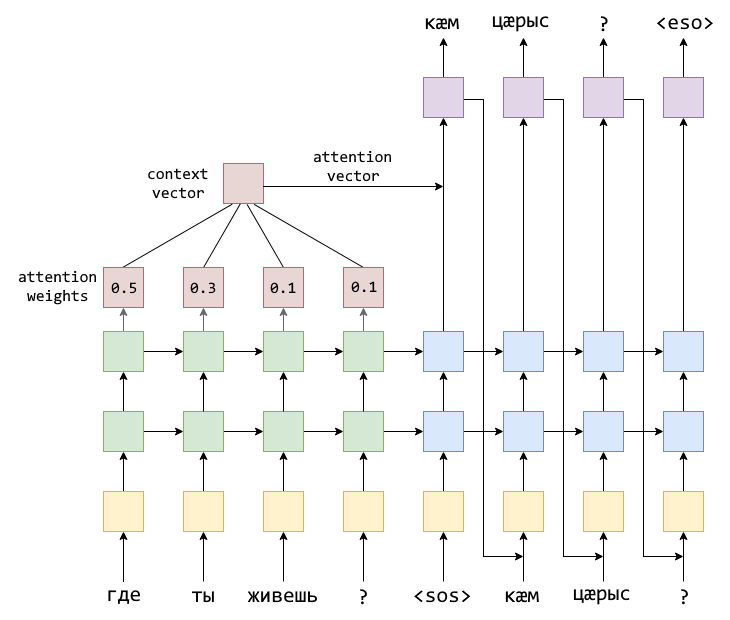
\includegraphics[width=0.75\textwidth]{img/Model.png}
		\caption{Encoder-Decoder Seq2Seq модель, с механизмом Attention}
	\end{figure}
	
	\subsection{Обучение}
	
	Последним этапом построение модели машинного перевода является определение механизма обучения. Нейронные модели Seq2Seq обучаются предсказывать распределения вероятностей следующего элемента последовательности с учетом предыдущего контекста. На каждом шаге нужно максимизировать вероятность, которую модель присваивает правильному элементу. 
	
	Формально, давайте представим, что у нас есть обучающий экземпляр с входом  $X = \{ x_0, ... , x_T \}$ и целевой выход $Y = \{ y_0, ... , y_T \}$. Затем на временном шаге $t$ модель предсказывает распределение вероятностей $P^{(t)} = P(*|y_0, ..., y_{t - 1}, x_0, ..., x_{T})$. Основная цель на этом этапе, чтобы модель присваивала вероятности 1 правильному элементу $y_t$ и 0 остальным.
	
	В таких случаях обычно использует максимальное логарифмическое правдоподобие (MLE) или категориальную кросс-энтропию (CCE) в качестве целевой функции обучения, которая является используемым методом оценки параметров распределения вероятностей. Формально, учитывая обучающий набор $ \mathcal{D} = \{\textlangle x(s), y(s) \textrangle\}_{s=1}^S $, целью обучения является поиск набора параметров модели $\theta$, которые максимизируют логарифмическую вероятность на обучающем наборе:
	
	$$
	    \hat{\theta}_{\text{loss}} = argmax(\mathscr{L}(\theta)),
	$$

    где логарифмическая вероятность определяется как:
    
    $$
      \mathscr{L(\theta)=\sum_{s=1}^S log(P(y^{(s)}|x^{(s)};\theta))}  
    $$
    
    Благодаря алгоритму обратного распространения ошибки можно эффективно вычислить градиент $\mathscr{L}$ относительно $\theta$ (параметров модели). При обучении моделей NMT обычно используется алгоритм стохастического градиентного спуска (SGD). Вместо вычисления градиентов на полном обучающем наборе SGD вычисляет функцию потерь и градиенты на маленькой части обучающего набора. Простой оптимизатор SGD обновляет параметры модели NMT с помощью следующего правила:
    
    $$
        \theta \leftarrow \theta - \alpha \nabla \mathscr{L}(\theta)
    $$
    
    где $\alpha$ - скорость обучения. При правильно выбранной скорости обучения параметры NMT гарантированно сходятся к локальному оптимуму. На практике оказывается, что адаптивные оптимизаторы скорости обучения, такие как Adam \cite{14}, значительно сокращают время обучения, а точность почти не снижается.
    
	\subsection{Вывод}
	
	После полного прохождения всех этапов, остается понять как сгенерировать перевод из полученной модели. В идеале хотелось бы найти целевую последовательность $y'$, которая максимизирует прогноз модели $P(y|x=X;\theta)$ в качестве перевода, где $X$ - входная последовательность. Однако из-за непомерно большого пространства поиска найти перевод с наибольшей вероятностью затратно. Поэтому NMT обычно использует локальные алгоритмы поиска, такие как Beam search \cite{8}, для поиска наилучшего перевода.
	
	Beam search - это классический алгоритм локального поиска, который широко используется в NMT. Алгоритм Beam search отслеживает $k$ состояний на этапе вывода. Каждое состояние представляет собой кортеж $(y_0, y_1, ..., y_t, v)$, где $y_0, y_1, y_2, ..., y_t$ является кандидатом на перевод, а $v$ - логарифмическая вероятность кандидата. На каждом шаге генерируются все преемники всех $k$ состояний, но выбираются только верхние $k$ преемников. Алгоритм обычно завершается, когда шаг превышает заранее определенное значение или найдено $k$ полных преобразований. Следует отметить, что поиск по лучу превратится в жадный поиск, если $k = 1$.
	
	\begin{figure}[ht!]
		\centering
		\captionsetup{justification=centering}
		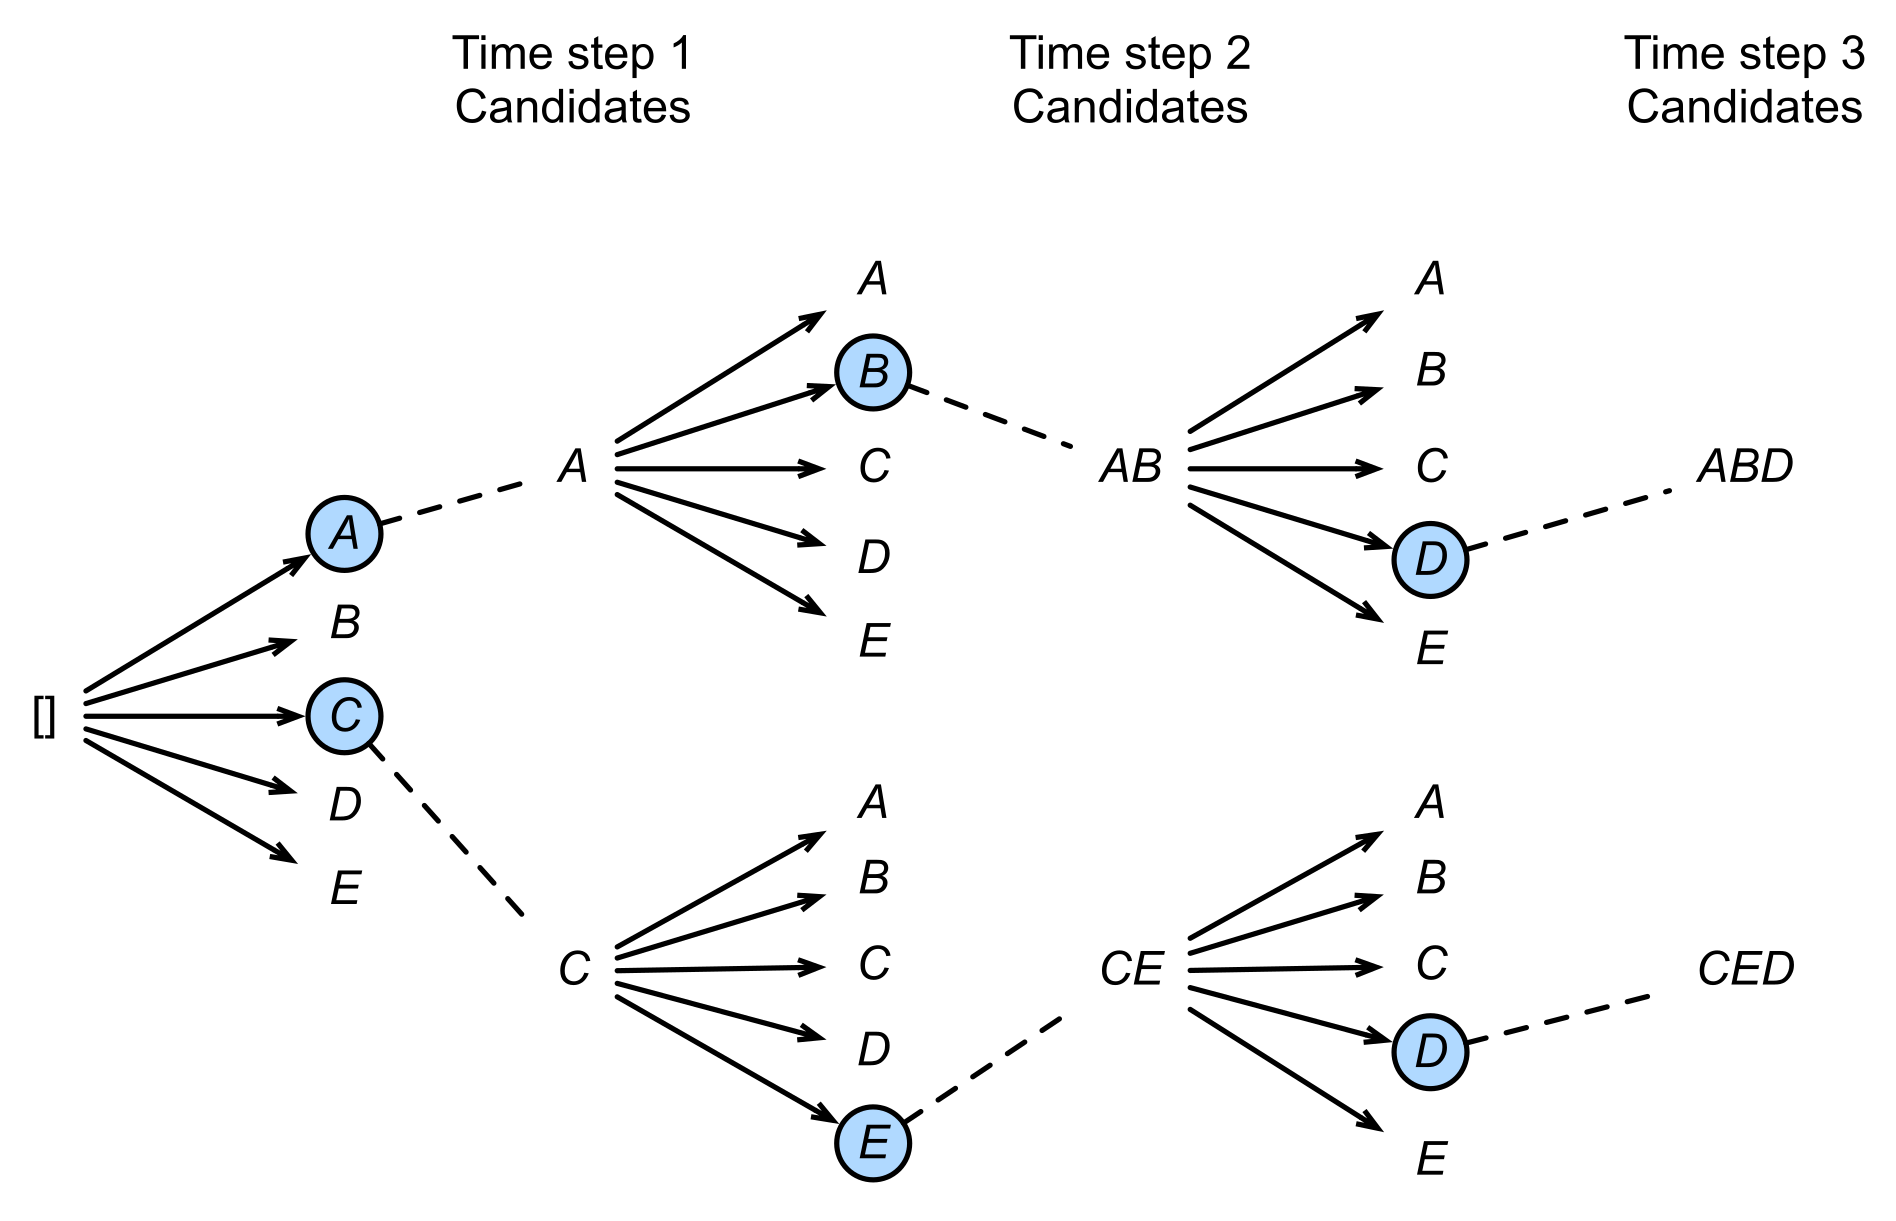
\includegraphics[height=90mm]{img/beam-search.png}
		\caption{Схема алгоритма Beam Search}
	\end{figure}
	
	\section{Attention}
	
	Механизм внимания (Attention mechanism) - это часть нейронной сети для поиска взаимосвязей между различными частями входных и выходных данных. Несмотря на то, что нейронные сети довольно сложно интерпретировать. Объяснить внутренности в понятных человеку терминах часто невозможно. Однако придуманный механизм внимания, абсолютно интуитивно понятный \cite{16}..
    
    Успех использования этого подхода в задаче машинного перевода обусловлен лучшим выводом закономерностей между словами находящимися на большом расстоянии друг от друга. Несмотря на то, что LSTM и GRU блоки используются именно для улучшения передачи информации с предыдущих итераций RNN их основная проблема заключается в том, что влияние предыдущих состояний на текущее уменьшается экспоненциально от расстояния между словами, в то же время механизм внимания улучшает этот показатель до линейного \cite{17}.
    
    RNN используются при обработке данных, для которых важна их последовательность. В классическом случае применения RNN результатом является только последнее скрытое состояние $h_n$, где $n$— длина последовательности входных данных. Использование механизма внимания позволяет использовать информацию полученную не только из последнего скрытого состояния, но и любого скрытого состояния $h_t$ для любого $t$.
    
    В дальнейшем Decoder использует внимание для выборочного фокусирования на частях входной последовательности. Прежде чем почитать сам вектор внимания нужно вычислить функцию оценки $score(h_t, s_k), k = 0, ... n$, где $h_t$ - одно скрытое состояние Decoder, а $s_k$ - все состояния Encoder на шаге $k$.
	
	Функцию оценки для каждого скрытого состояния Encoder объединяются и представляются в виде одного вектора, а затем передаются в функцию активации softmax, отсюда получается новый вектор. 
	
	Вектор выравнивания - это вектор, имеющий ту же длину, что и исходная последовательность. Каждое из его значений представляет собой оценку (или вероятность) соответствующего слова в исходной последовательности. Векторы выравнивания задают веса на выходе Encoder. С помощью этих весов Decoder решает, на чем сосредоточиться на каждом временном шаге.
	
	Скрытые состояния Encoder и их соответствующие оценки (веса внимания) умножаются для формирования контекстного вектора. Вектор контекста используется для вычисления в дальнейшем конечного выходного сигнала Decoder.
		
	\begin{figure}[ht!]
		\centering
		\captionsetup{justification=centering}
		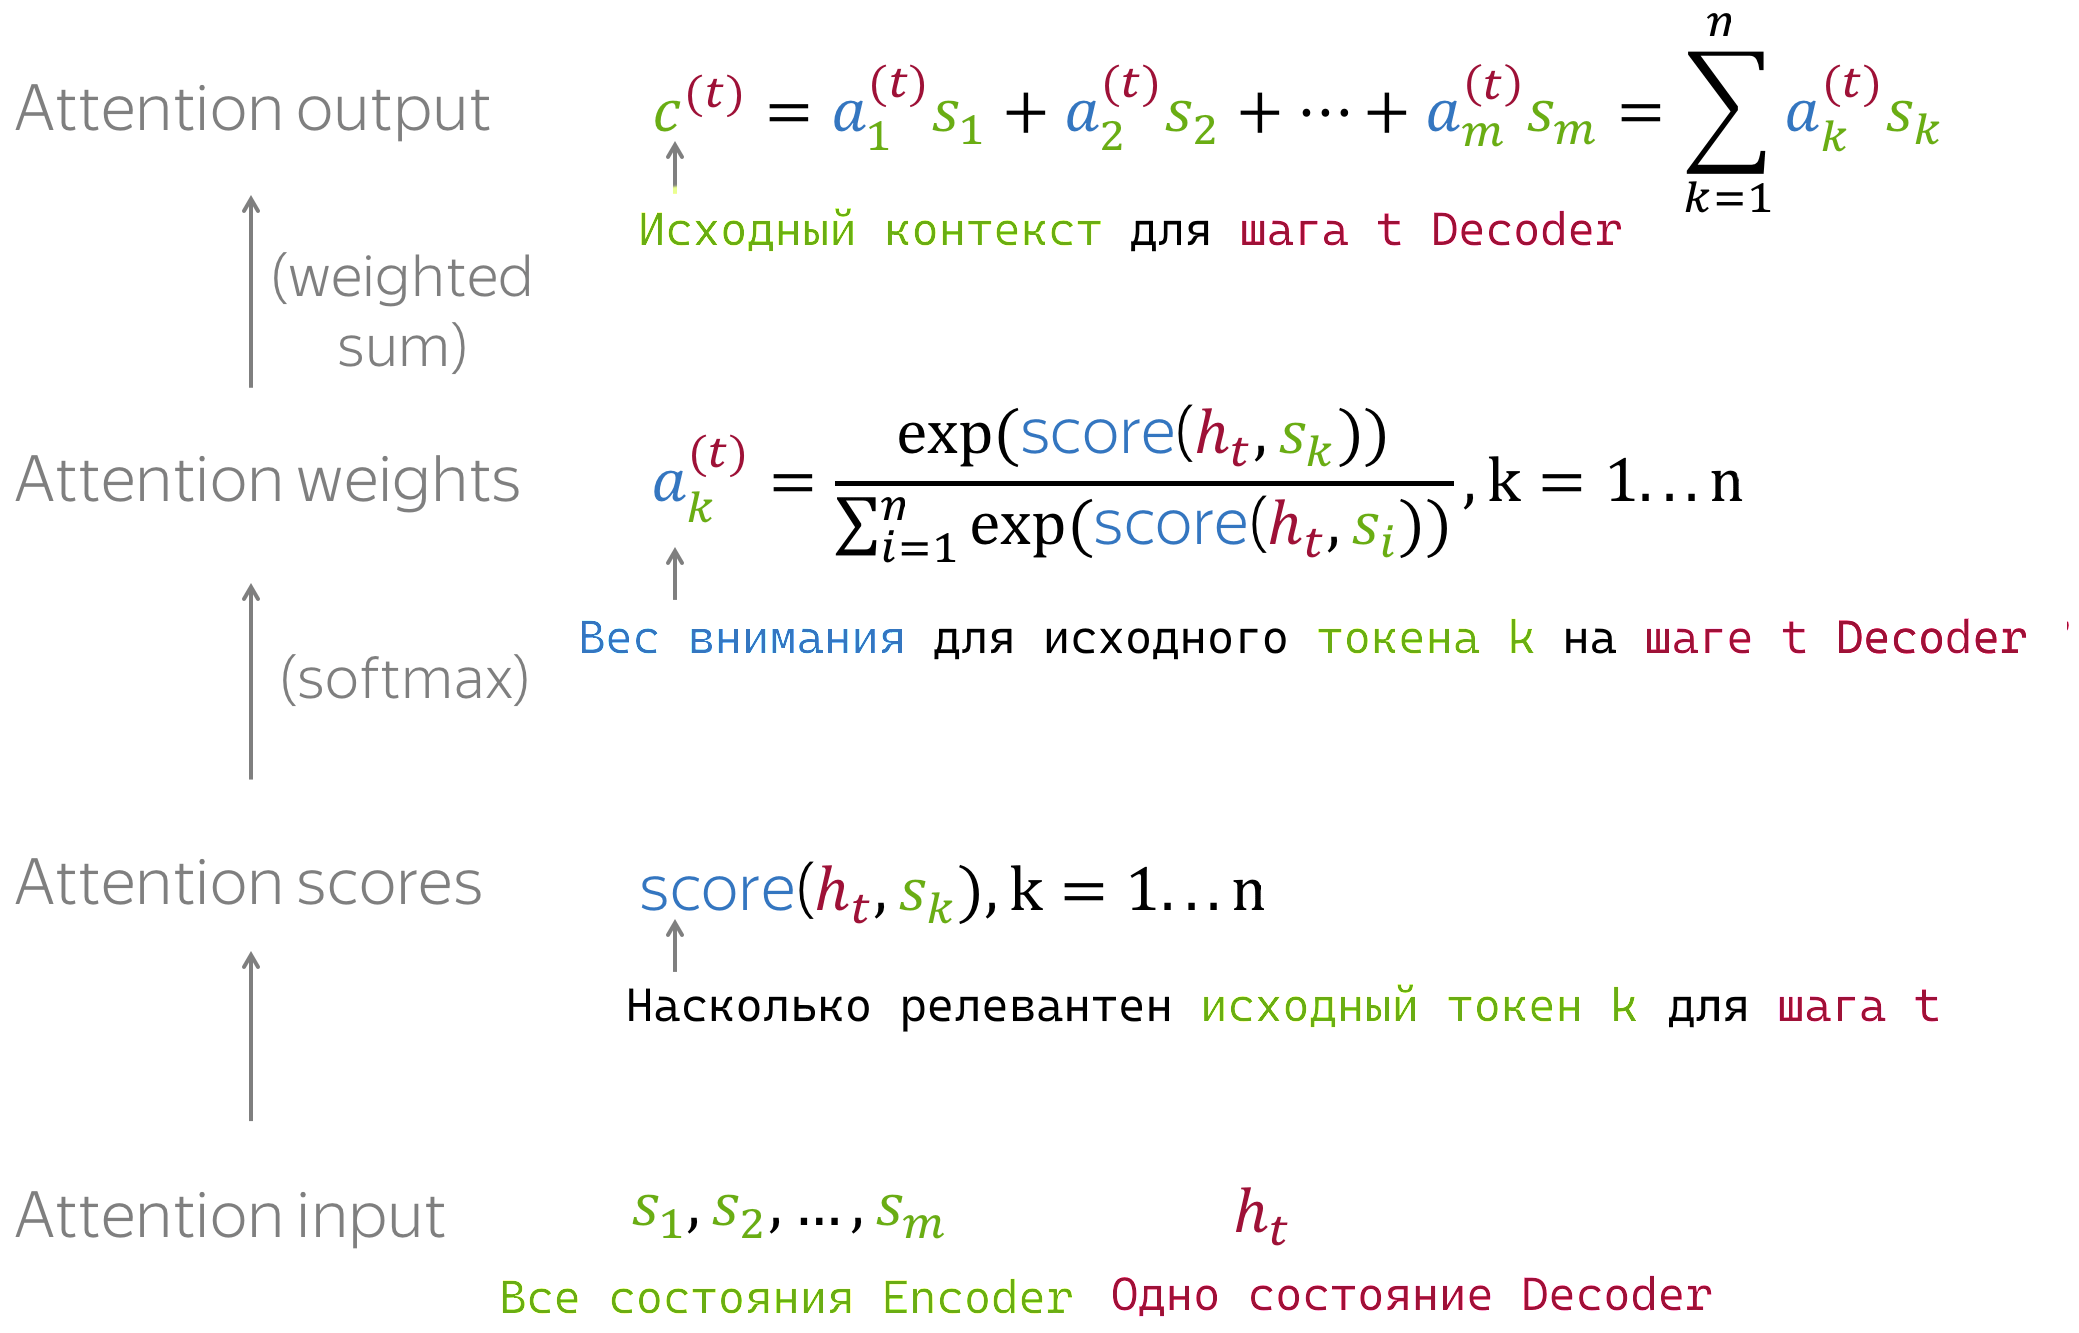
\includegraphics[height=70mm]{img/Attetion.png}
	\end{figure}
	
	\clearpage

	\section{Реализация модели Seq2Seq в TensorFlow}
	
	\subsection{Поиск данных}
	
	Прежде чем переходить к созданию собственной модели, стоит так же побеспокоиться о данных. От качества входных пар (предложение, перевод) зависит и результат модели. Стоит уделить довольно много внимания на данный аспект.
	
	В процессе работы были построены несколько моделей на основе двух дата-сетов с парами языков:
    
    \begin{table}[h]
        \centering
        \begin{tabular}{|c|c|} 
        \hline
        \textbf{Тип языковой пары}                                       & \textbf{Количество}  \\ 
        \hline
        Русский язык $\shortrightarrow$ Английский язык & 100 000              \\ 
        \hline
        Русский язык $\shortrightarrow$ Осетинский язык & 1 878                \\
        \hline
        \end{tabular}
        \caption{Количество пар в датасетах}
    \end{table}
    
    Так как краеугольным камнем в поставленной задаче является качество и количество данных, обойтись одной парой языков недостаточно. Поэтому все модели проверены на двух дата-сетах. Большой дата-сет (\textit{RUS $\shortrightarrow$ ENG}), даст возможность минимизировать ошибки в структуре построения самих моделей. В свою очередь это увеличит шанс на удачную работу таких же моделей, но с другой парой поменьше (\textit{RUS $\shortrightarrow$ OSS}). Таким образом можно сосредоточься только на самих параметрах модели и этапах её обучения, уделяя меньше времени на изменение самой структуры модели Seq2Seq.
	
	Весь материал, который в последствие был переработан в дата-сеты, был собран на данных ресурсах: 
	
	\begin{enumerate}
		\item \textit{RUS $\shortrightarrow$ ENG} - Дата-сет предложений с переводом с русского языка на английский.
		\begin{enumerate}
			\item ManyThings.org - Двуязычные Пары предложений, разделенные табуляцией. 
			Это выбранные пары предложений из проекта Tatoeba. \\ 
			\url{http://www.manythings.org/anki/}
		\end{enumerate}
		\item \textit{RUS $\shortrightarrow$ OSS} - Дата-сет предложений с пользовательским переводом с русского языка на осетинский.
		Кусочно собран с разных ресурсов, таких как:
		\begin{enumerate}
			 \item Проект \textit{Tatoeba} - обширная база данных предложений и их переводов, постоянно пополняющаяся усилиями тясяч добровольных участников. \\ \url{https://tatoeba.org/ru/downloads}
			 \item Проект \textit{Биоингвӕтӕ} - Билингвы подготовлены для чтения с помощью электронных словарей программы Lingvo. \\ \url{https://ironau.ru/bilingva/index.htm}
			 \item Ф.М. Таказов - Краткий русско-осетинский разговорник. \\ \url{https://ironau.ru/takazov/phrasebook2.htm}
			 \item Ф.М. Таказов - Самоучитель осетинского языка. \\ \url{https://ironau.ru/takazov/index.htm}
 		\end{enumerate}
	\end{enumerate}
	
	\clearpage
	
	\subsection{Обработка данных}
	
	В процессе работы с данными были обнаружены некоторый перечень проблем. 
    Датасет \textit{RUS $\shortrightarrow$ ENG}, почти не имеет в себе проблем, кроме одной. В некоторых парах используется сокращения принятые в английском языке (Например: I am $\shortrightarrow$ I'm). Данная проблема не была решена. Поэтому в статье данная проблема игнорируется.
    
    Так же в датасете \textit{RUS $\shortrightarrow$ OSS} были обнаружены символы «æ» (Код: 1237) и «æ»(Код: 230). Данная буква несет в себе одинаковую смысловую нагрузку в языке, следовательно просто заменим все символы на «æ» с кодом 230 (т.к. аналогичный символ используется на Осетинской Википедии). 
    
    Еще есть проблема с символом «тире». Два вида символов «—» и «-», тоже несут в себе одинаковую ценность, связи с этим заменяем их на какое-то одно в данном случае на второй символ из представленных («-»).
	
	\begin{lstlisting}[language=iPython]
	
	\end{lstlisting}

    \clearpage
	
	\section{Заключение}
	
	В работе рассмотрена модель машинного перевода Seq2Seq c использованием нескольких архитектур рекуррентных нейронных сетей (LSTM и GRU). На практике полученные модели были хороши для работы с последовательностями, однако возникают трудности при запоминании долгосрочных зависимостей.
	
	В качестве главной цели этой работы, стоит реализация модели машинного перевода, а так же оценка качества полученного результата и его зависимостей от параметров модели на этапе обучения.
	
	\clearpage
	
	\addcontentsline{toc}{section}{Список используемой литературы}
	
	\begin{thebibliography}{}
		\bibitem{1}  Michael I. Jordan	-	Serial Order: A Parallel Distributed Processing Approach; 1986. 
		
		\url{https://cseweb.ucsd.edu/~gary/PAPER-SUGGESTIONS/Jordan-TR-8604-OCRed.pdf}
		
		\bibitem{2}  S. Hochreiter, J. Schmidhuber	-	Long Short-Term Memory; 1997.
		
		\url{https://www.researchgate.net/publication/13853244_Long_Short-term_Memory}
		
		\bibitem{3}  Junyoung Chung, Caglar Gulcehre, KyungHyun Cho, Yoshua Bengio	-	Empirical Evaluation of Gated Recurrent Neural Networks on Sequence Modeling; 2014.
		
		\url{https://www.researchgate.net/publication/269416998_Empirical_Evaluation_of_Gated_Recurrent_Neural_Networks_on_Sequence_Modeling}
		
		\bibitem{4} J. Elman	-	Finding Structure in Time; 1990.
		
		\url{http://psych.colorado.edu/~kimlab/Elman1990.pdf}
		
		\bibitem{5} Ilya Sutskever	-	Training recurrent neural networks; 2013.
		
		\url{https://www.cs.utoronto.ca/~ilya/pubs/ilya_sutskever_phd_thesis.pdf}
		
		\bibitem{6} Ян Гудфеллоу, Иошуа Бенджио, Аарон Курвилль	-	Глубокое обучение; М.: ДМК Пресс, 2018 - 652c. 
		
		\bibitem{7} С. Николенко, А. Кадурин, Е. Архангельская	-	Глубокое обучение;  СПб.: Питер, 2018 - 480c.
		
		\bibitem{8} Alex Sherstinsky	-	Fundamentals of Recurrent Neural Network (RNN) and Long Short-Term Memory (LSTM) Network; 2018.
		
		\url{https://www.researchgate.net/publication/326988050_Fundamentals_of_Recurrent_Neural_Network_RNN_and_Long_Short-Term_Memory_LSTM_Network}
		
		\bibitem{9} Zachary Chase Lipton	-	A Critical Review of Recurrent Neural Networks for Sequence Learning; 2015.
		
		\url{https://www.researchgate.net/publication/277603865_A_Critical_Review_of_Recurrent_Neural_Networks_for_Sequence_Learning}
		
		\bibitem{10} Ri Wang, Maysum Panju, Mahmood Reza Gohari -   Classification-based RNN machine translation using GRUs; 2017
		
		\url{https://www.researchgate.net/publication/315570520_Classification-based_RNN_machine_translation_using_GRUs}
		
		\bibitem{11} Tomohiro Fujita, Zhiwei Luo, Changqin Quan, Kohei Mori - Simplification of RNN and Its Performance Evaluation in Machine Translation; 2020
		
		\url{https://www.jstage.jst.go.jp/article/iscie/33/10/33_267/_pdf/-char/en}
		
		\bibitem{12} Sainik Kumar Mahata, Dipankar Das and Sivaji Bandyopadhyay -  MTIL2017: Machine Translation Using Recurrent Neural Network on Statistical Machine Translation; 2018
		
		\url{https://www.researchgate.net/publication/325456613_MTIL2017_Machine_Translation_Using_Recurrent_Neural_Network_on_Statistical_Machine_Translation}
		
		\bibitem{13} Zhixing Tan, Shuo Wang, Yang Zonghan, Gang Chen - Neural Machine Translation: A Review of Methods, Resources, and Tools; 2020
		
		\url{https://www.researchgate.net/publication/348079690_Neural_Machine_Translation_A_Review_of_Methods_Resources_and_Tools}
		
		\bibitem{14} Timothy Mayer, Ate Poortinga, Biplov Bhandari, Andrea P. Nicolau, Kel Markert, Nyein Soe Thwal, Amanda Markert, Arjen Haag, John Kilbrideh, Farrukh Chishtie, Amit Wadhwai, Nicholas Clintonj, David Saah - Deep Learning approach for Sentinel-1 Surface Water Mapping leveraging Google Earth Engine; 2021
		
		\url{https://www.researchgate.net/publication/355005296_Deep_Learning_approach_for_Sentinel-1_Surface_Water_Mapping_leveraging_Google_Earth_Engine}
		
		\bibitem{15} Kishore Papineni, Salim Roukos, Todd Ward, Wei-Jing Zhu - BLEU: a Method for Automatic Evaluation of Machine Translation; 2002
		
		\url{https://www.researchgate.net/publication/2588204_BLEU_a_Method_for_Automatic_Evaluation_of_Machine_Translation}
		
		\bibitem{16} Ashish Vaswani, Noam Shazeer, Niki Parmar, Jakob Uszkoreit, Llion Jones, Aidan N. Gomez, Lukasz Kaiser, Illia Polosukhin - Attention Is All You Need
		
		\url{https://arxiv.org/abs/1706.03762}
		
		\bibitem{17} Giuliano Giacaglia - How Transformers Work
		
		\url{https://towardsdatascience.com/transformers-141e32e69591}
		
		\bibitem{18} Dzmitry Bahdanau, Kyunghyun Cho, Yoshua Bengio - Neural Machine Translation by Jointly Learning to Align and Translate
		
		\url{https://arxiv.org/abs/1409.0473}
		
		\bibitem{19} Rohan Jagtap - TransCoder: Facebook’s Unsupervised Programming Language Translator
		
		\url{https://medium.com/swlh/transcoder-facebooks-unsupervised-programming-language-translator-10b82d1c7a9e}
		
		\bibitem{20} Викиконспекты ИТМО
		
		\url{https://neerc.ifmo.ru/wiki/index.php?title=Машинное_обучение}
		
		\bibitem{21} Mani Wadhwa - seq2seq model in Machine Learning, 2021
		
		\url{https://www.geeksforgeeks.org/seq2seq-model-in-machine-learning/}
		
		\bibitem{22} LSTM – сети долгой краткосрочной памяти
		
		\url{https://habr.com/ru/company/wunderfund/blog/331310/}
	\end{thebibliography}
\end{document}


% \begin{lstlisting}[language=iPython]

% \end{lstlisting}